\documentclass[10pt,twocolumn,letterpaper]{article}
\usepackage{cvpr}
\usepackage{times}
\usepackage{graphicx}
\usepackage{amsmath}
\usepackage{amssymb}
\usepackage{fancyvrb}
\usepackage{fvextra}
%\usepackage{underscore}
\usepackage[pagebackref=true,breaklinks=true,colorlinks,bookmarks=false]{hyperref}
\hypersetup{
    colorlinks=true,
    linkcolor=blue,
    urlcolor=blue,
}
\def\GroupID{DL\_DT\_Explore} % <------- ENTER YOUR COMP 691 group number here

\begin{document}
\title{LEARNING FROM LIMITED DATA WITH RESOURCE CONSTRAINTS}
\author{ Hussein Abdallah \and Trong-Tuan Tran \and Manh-Quoc-Dat Le}
\maketitle


%------------------------------------------------------------------------
\section{Introduction}

Learning with limited data are one of the interesting aspects of Deep Learning (DL) in Machine Learning (ML) field in general. Through this project we have a chance to experience this challenge in two different contexts.   

%State your goal by giving give an example of the data you're working with and an example of the kind of prediction you hope to achieve. 
\subsection{Project description:}
%Text compression could be considered an indicator of intelligence, in the context that if a compressor can perform efficiently, it would probably a smart one. Moreover, compressing the Wikipedia's text data is some how closed to understanding human's knowledge. We evaluate our work on \textit{\textbf{EnWik9}}, which is a 1GB snapshot of English Wikipedia text in XML format and the benchmark data for the Hutter Prize \cite{hutter}. Apart from XML tags, an example of data looks like:


\paragraph{Challenge 1:}
 %The main goal of our project is to create a lossless text compression program which could be able to deliver an acceptable compression ratio and execute in a reasonable amount of time. By saying "acceptable ratio", we mean that our compressor should be able to achieve a better bits per input byte (or b.p.b) compared to standard compressors using zero-order Markov models (such as Huffman Codes, gzip, etc..), but certainly could not compete with the State of The Art model like CMix (\cite{cmix}) with much more complexity as well as longer training time, and "reasonable time" means shorter (de)compression time compared to cmix. Table~\ref{table:compress} summarizes performance of some popular compression algorithms on the entire Enwik9 dataset.
Few-sample learning on the CIFAR-10 dataset. We will consider a dataset with only 100 samples. For testing a larger dataset will be used (e.g. the CIFAR-10 test set).
The task is to train on 100 randomly selected (but class balanced) samples from the CIFAR-10 training set.

Final evaluation: In the final evaluation your model will be run on 5 random instances of this problem. Evaluation will occur both on the CIFAR-10 test set and other data which will not be revealed at the moment. There is also a CodaLab competition in this challenge 1 and the CodaLab environment only supports CPU, not GPU.

Time constraint for challenge 1 is 2 hour model running time in GPU.

\paragraph{Challenge 2:}
Consider the same exercise with challenge 1 but now with the ability to use an external data or models not trained on CIFAR-10 from the pytorch model repository or to train your own model on external data (you may not train a model on CIFAR-10 dataset or any derivative using these images.
Teams may consider for example various forms of fine-tuning, meta-learning, semi-supervised learning with an external dataset and other related ideas).

For both challenges, during development phase, the team should train and evaluation on the train set, while the final result of training and testing on CIFAR-10 Test set need to be reported with the average and standard deviation. This should be done on a minimum of 3 splits. Each split should use 100 training samples and a separate 2000 samples for testing as done in the test bed when sampling from CIFAR-10 Train set.

 \subsection{Goals}
 \label{subsection:intro_goals}
 \begin{itemize}
  \item For challenge 1, due to the present of the competition in CodaLab \cite{CodaLab_comp}, our goal is not just simply reaching max test accuracy, but there is more things to be taken into account. Due to limited sample size (100 samples without using pre-trained model) and randomness, variation of model performance between each running instance plays a big role. From early development phase the team observed that it's not so difficult to increase model accuracy when it has not reached its full potential, but the problem is there is too much variances on the final test accuracy between runs within the same code and hyper-parameters, as well as there can be huge differences in performance between running in the training set from our test-bed v.s. running in CodaLab test set, which will be discussed further in the implementation and result section \ref{subsubsection:challenge1_result}. Another factor to consider is execution speed: since the CodaLab environment for the competition can support running with CPU but not GPU and the maximum execution time allowed is 2 hours, the submitted model on CodaLab should be able to running in CPU within the limited time frame. Hence, our goal for challenge 1 is to achieve the best test accuracy with acceptable execution time (not much longer than the provided baseline CNN model), and most importantly, \textbf{the model should have maximized regularization, or minimized variation across running instances for both local and CodaLab execution}.       
  \item For challenge 2, many pre-trained models are found that you can start with to classify your few samples problem. Many of them are trained with ImageNet data-set \cite{deng2012imagenet} that has more than 20,000 categories including their annotations. The problem here is which model is more suited to your problem and how deep that model is to generalize well using your limited data. In addition to model selection, many questions will appear that need  more investigations such as: how to find similar classes data-set to train your model with? What data augmentation and fine tuning well suite your data? What are optimization techniques you need to look at it carefully to achieve higher accuracy? And finally, how much resource and time your model will need during training and inference time?. Thus, our goal for challenge 2 is to show how a very deep convolution neural network can be used to learn from small data-set like CIFAR-10 with few samples with availability of using  external data to achieve higher accuracy with low variance.

  
\end{itemize}
 
 
\subsection{CIFAR-10 Dataset} 
CIFAR-10 dataset \cite{CIFAR-10} is an abbreviation of Canadian Institute For Advanced Research. It is one of the most frequently used datasets for training machine learning (ML) models and computer vision algorithms. According to Wikipedia \cite{wiki:cf10}, CIFAR-10 dataset  consists of 60,000 32x32 color images in 10 different classes, which are airplane, automobile, bird, cat, deer, dog, frog, horse, ship, and truck. There are 6,000 images per class. From the total of 60,000 images in the dataset, CIFAR-10 is split into training and testing sets, which contain 50,000 and 10,000 images, respectively. As the name already implied, training dataset is used for researchers to design and implement their algorithms/approaches and testing set is used for evaluating their solutions/models.

CIFAR-10 image set is mainly used to teach a computer how to recognize or classify objects through photos. Due to low resolution of images (32x32) in the dataset, CIFAR-10 is a reasonable choice for data scientists/engineers could come up with different algorithms or models rapidly to conclude which is the best. There are numerous models based on Convolutional Neural Network (CNN) \cite{krizhevsky12_cnn} having high accuracies at classifying images in the CIFAR-10 dataset.
 
\subsection{CINIC-10 Dataset} 
CINIC-10 is an augmented extension of CIFAR-10. It contains the images from CIFAR-10 (60,000 images, 32x32 RGB pixels) and a selection of ImageNet database images (210,000 images downsampled to 32x32). It was compiled as a 'bridge' between CIFAR-10 and ImageNet, for benchmarking machine learning applications. It is split into three equal subsets - train, validation, and test - each of which contain 90,000 images.
\cite{cinic-10}



%------------------------------------------------------------------------
\section{Literature Review}
We categorize this literature review into 3 parts: papers that are applied or relevant for both challenges and then papers we applied separately for each challenge.  


\subsection{Papers applied for both challenges}
\label{subsection:literature-both-challenges}
\paragraph{A Survey on Image Data Augmentation for Deep Learning:}
According to \cite{data_aug_survey_2019}, Deep Learning Models have made a tremendous progress in discriminative tasks in various domains and one of them is computer vision. This has been fulfilled by the rapid growth of deep network architectures, powerful computation, and access to big data. Deep neural networks have been effectively utilized in Computer Vision tasks, such as object recognition, image classification, and image segmentation thanks to the success of convolutional neural networks (CNNs). Currently, there are large number of studies with the purpose of improving benchmarks in computer vision tasks by designing algorithms based on deep CNNs. Improving generalization of the state-of-the-art models is one of the most difficult challenges. Models, that are poor generalization, have overfitting occurrence in the training data. Data Augmentation is one of the solutions to build appropriate deep learning models with lower validation errors as well as training errors. The augmented data will represent a more complete set of possible data points, that will minimize the gap between training set and validation set, as well as testing sets in the future.

Data augmentation will artificially enlarge the training set size by either \textbf{data warping} or \textbf{oversampling}. \textbf{Data warping} means transforming existing data (images) but preserving their labels. There are several techniques categorized as data warping augmentation, such as geometric and color transformations, random erasing, adversarial training, and neural style transfer. \textbf{Oversampling} means creating more synthetic data points and adding them to the training set. This category consists of mixing images, feature space augmentations, and generative adversarial networks (GANs).

\textbf{Image Data Augmentation Techniques:} In this survey, the authors listed the following techniques: geometric transformations, color space transformations, kernel filters, mixing images, random erasing, feature space augmentation, adversarial training, GAN-based augmentation, neural style transfer, and meta-learning schemes.

\begin{enumerate}
    \item \textbf{Data Augmentations based on basic image manipulations:}
    \begin{itemize}
        \item \textbf{Geometric transformations:} In this section, the authors described different augmentations based on geometric transformations and a number of other image processing functions. They also described these augmentations in the context of “safety” application. That means the likelihood of preserving the label post-transformation of a data augmentation method.
        \begin{itemize}
            \item \textbf{Flipping:} Horizontal axis flipping is much more being used than flipping the vertical axis. This method has been proven effective on datasets such as CIFAR-10 and ImageNet.
            \item \textbf{Color space:} Digital image data is usually represented as a tensor with dimension of height x width x color channels. A simple color augmentation method is to isolate a single-color channel, such as R, G, or B. Doing so, we could increase or decrease the brightness of an image by performing matrix operations on these RGB matrices.
            \item \textbf{Cropping:} Cropping images is a practical processing step for data as images. This technique is useful when dealing with images that have mixed height and width dimensions by cropping a central patch of each image.
            \item \textbf{Rotation:} Rotation augmentations are performed by rotating an image right or left on an axis between 1o and 359o. By using this method, there is a notice that as the rotation degree increases, the label of the image is no longer preserved post-transformation.
            \item \textbf{Translation:} Shifting images left, right, up, or down could be a powerful method to avoid positional bias in the data.
            \item \textbf{Noise injection:} Noise injection is an augmentation method that injects a matrix contains random values, which drawn from a Gaussian distribution, into image dataset. This could encourage CNNs learn more robust features.
        \end{itemize}
        \item \textbf{Color space transformations:} Image data is represented as 3 stacked matrices, where each of size height x width. Lighting biases are the most regularly existing challenges to image recognition problems. Therefore, color space transformation is also known as photometric transformation. Amending the color distribution of images could be a great solution for lighting challenges in testing data. Image representations in datasets can also be simplified by converting the RGB matrices into a single grayscale image. There are some additional representations for digital color such as HSV (Hue, Saturation, and Value). In our approach, we mainly utilize HSV representation and grayscale image transformation.
        \item \textbf{Kernel Filters:} Kernel filter is a well-known technique in image processing to sharpen and blur images. The way the method works is sliding an n x n matrix across an image with either a Gaussian blur filter, which causes the image blurrier, or a high contrast horizontal or vertical edge filter, which will make the image sharper along edges. Kang \textit{et al.} \cite{kang2017patchshuffle} made experiments with a unique kernel filter that randomly switches the pixel values in an n x n sliding window. They call this technique PatchShuffle Regularization. They achieved a 5.66\% error rate on CIFAR-10 dataset compared to an error rate of 6.33\% without using the technique.
        \item \textbf{Mixing Images:} Mixing images together by averaging their pixel values seems not a useful transformation method to a human, but it brings amazing results to classification models, conversely. Ionue \cite{inoue2018data} showed that pairing of samples could be built up into an effective augmentation approach. Ionue performed this SamplePairing Data Augmentation technique on the CIFAR-10 dataset, and it brought up an incredible result by reducing the error rate from 8.22 to 6.93\%. However, this was not the final result Ionue could achieve. He/she found a better result, which was from 43.1 to 31.0\% in error rate, when testing a reduced in size of the dataset, that reduced CIFAR-10 to 1,000 samples with 100 samples for each class. This achievement demonstrated that the SamplePairing technique has been suitable for limited datasets.
        \item \textbf{Random erasing:} Random erasing is another interesting data augmentation technique that was invented by Zhong \textit{et al.} \cite{zhong2017random}. This method could be seen as analogous to dropout, except occurring in the input data space rather than in the network architecture. The technique works by randomly selecting an n x m patch of an image and masking it with either 0s, 255s, mean pixel values, or random values. The researcher achieved an error rate reduction from 5.17 to 4.31\% on the CIFAR-10 dataset and the best patch masked values found to be random ones.
    \end{itemize}
    \item \textbf{Data Augmentations based on Deep Learning:} In this category, there are 5 augmentation techniques including feature space augmentation, adversarial training, GAN-based augmentation, neural style transfer, and meta-learning schemes. In our approaches, we have not used this category of technique, so we just listed them out for introductory.
\end{enumerate}

Some augmentation techniques enlighten how an image classifier could be improved, while others do not. For example, it is easy to explain the advantage of horizontal flipping or random cropping. On the contrary, it is unclear why mixing images together technique such as PatchShuffle regularization or SamplePairing is so powerful. An interesting characteristic of augmentation methods is their ability to combine together. For example, the random erasing technique could be bundle up with any of other augmentation methods. An interesting question for practical data augmentation is how to determine post-augmented dataset size. There is no specific way to specify which ratio of original to final dataset size would make the model perform the best. Additionally, there is also no exact method for finding the best strategy to combine data warping and oversampling techniques. All the augmentation techniques perform best under the assumption that training and testing datasets drawn from the same distribution.

In this project, we applied most of the data augmentations based on basic image manipulations, which will be discussed later in Section \ref{section:method-and-implementation}.

\paragraph{Structural Analysis and Optimization of Convolutional Neural Networks with a Small Sample Size}: In \cite{dsouza_structural_2020}, D’souza \textit{et al.} conducted a throughout experiment to gain some insights on the influence of network structure on image classification performance using Convolutional Neural Networks (CNN) \cite{krizhevsky12_cnn} in the small data context, with the motivation that not all image training samples are abundantly available, especially with some specific application domains. 

With the speedy growth of available computation resources and Big Data era, more and more bigger, deeper models leveraging CPU, GPU and TPU show a common generalization principle that the deeper model and the more data feed in, the networks would perform better. However, those deep networks were developed under the assumption that the data samples would be sufficiently high enough, while there are huge amount of real-world applications having very limited sample size. "Small data" is consider when there are less than 5000 samples in the dataset, and some obvious applications that have access to limited data are medical images (including MRI, CT, ultrasounds, etc..).   

After the experiments on VC-dimensions \cite{wiki:vc-dimension} of different model structure generated, the author defined some best network structure for small datasets such as MNIST, CIFAR-10 and gave the arguments that deeper model are not always better. Another conclusion was that the optimal model structure depends on the data's nature, not so much on the data size.

We base on some conclusion of this article to decide on our model to be used for challenge 1.

\paragraph{Improving multiclass classification by deep networks using DAGSVM and Triplet Loss:}  In \cite{AGARWAL2018_DAGSVM}, Agarwal \textit{et al.} suggests a new method of improving multi-class classification accuracy, mainly by replacing the softmax function and having a triplet loss with a SVM classifier implemented using Directed Acyclic Graph (aka DAGSVM). DAG is a graph of nodes arrangement organized in a hierarchical structure, and when each node represents a SVM (One vs One binary classifier). For a problem of N classes, the DAG have \(N(N-1)/2\) number of nodes, as shown in figure \ref{figure:dagsvm}. 

 \begin{figure}[h!]
   \centering
       \includegraphics[width=1\linewidth]{img/REPORT_dagsvm.jpg}
   \caption{Directed Acycli Graph (DAG)\label{figure:dagsvm}}
 \end{figure}

The author also use triplet loss to learn discriminative features before feeding into the SVM classifier, where the online triplet selection policy is to pick the negatives randomly but still make sure that the anchors in a mini-batch have the same contribution from both classes.

The experiments were performed on CIFAR-10 and STL-10 datasets, with applied augmentations like data cropping and horizontal flipping. 
Fine-tuning after 4k iteration, the models using DAGSVM exceeded test accuracy of the models using the same network but with Softmax output. 

In the discussion part, the authors found that when improving the performance of each individual binary classifier in the DAG, the overall solution also gets positive impact. Moreover, the model can also be extended to support a large number of classes, with just the negative impact on additional training time.

In our project, one of our approaches in challenge 1 was inspired by this paper (although it can be applied for both challenges like the deep metric learning method mentioned previously). Moreover, the notable thing to mention is that the default algorithm of the SVM classifier in Scikit-learn library that we are going to implement is also based on one-vs-one policy.



\subsection{Papers applied for challenge 1} 
\paragraph{Deep Learning on Small Datasets without Pre-Training using Cosine Loss:} Barz \textit{et al.} in \cite{cosine-loss}, have showed that applying the cosine loss function gives considerably better performance than using cross-entropy loss after softmax activation, which is the most common choice for classification problems, on limited dataset size with a small number of samples per class. They conducted experiments on 5 small image datasets including CUB, NAB, Stanford Cars, Oxford Flowers, MIT Indoor Scenes and one text dataset which is AG News.

To address the problem of learning from limited data, there is an enormous number of studies in the field of few-shot and one-shot learning. Specifically, models will learn features from a large training dataset so that they could perform well on it, later on taking these models to perform on a dataset with limited data for each class by using nearest neighbor approach. However, Barz et al. have solved the problem in a different way. They made a deep neural network classifier learning directly on small datasets, without pre-trained on external datasets. The cramped datasets they were training on even just have roughly between 20 and 100 data points per class. In addition to that, inspired by the work of Barz and Denzler \cite{8658633}, which used cosine loss to map images onto semantic class embedding derived from a hierarchy of classes in the context of image retrieval. Although the purpose of Barz and Denzler is to improve semantic consistency of image retrieval results, they also realized that classification accuracies were impressive on NAB dataset without pre-training. Barz and \textit{et al.} in \cite{cosine-loss} have shown that the reason behind the above circumstance is the cosine loss function and this loss function could be implemented in any limited dataset size to achieve remarkable classification accuracy than using traditional cross-entropy loss, just by embedding classes with one-hot vectors.

\textbf{Cosine Loss:} The cosine similarity between d-dimensional vectors $a,b \in \mathbb{R}^d$ is defined as:
\[
\sigma_{\cos}\left(a,b\right)=\cos{\left(a\angle b\right)}=\frac{\left\langle a,b\right\rangle}{\|a\|_2\cdot\|b\|_2} \ ,\qquad\qquad(1)
\]
where: \(\langle\cdot,\cdot\rangle\) denotes the dot product and \(\|\cdot\|_p\) denotes the \(L_p\) norm.
\newline

Let \(x\in\mathfrak{X}\) be an instance in the training set (images, text, etc.) and \(y\in\mathcal{C}\) be the class label of x from the set of classes \(\mathcal{C}=\{1,\ldots,n\}\). In addition to that, \(f_\theta:\mathfrak{X}\rightarrow \mathbb{R}^d\) denotes a transformation with model’s parameters \(\theta\) from the input space \(\mathfrak{X}\) into a d-dimensional Euclidean feature space by a deep neural network classifier. \(\psi: \mathbb{R}^d \rightarrow \mathcal{P} \ and \ \varphi: \mathcal{C} \rightarrow \mathcal{P}\) denotes the embedding features and classes into a common prediction space \(\mathcal{P}\), respectively.
\newline

Below is an example of a class representation as a one-hot vector:
\[
\varphi_{onehot}\left(y\right)=\left[{\underbrace{0\ldots0}}_{y-1\ times}\quad 1\quad {\underbrace{0\ldots0}}_{n-y\ times}\right]^\mathsf{T}.\left(2\right)
\]

Barz \textit{et al.} define the cosine loss function as:
\[
\mathcal{L}_{\cos}\left(x,y\right)=1-\sigma_{\cos}\left(f_\theta\left(x\right),\varphi\left(y\right)\right) \ .\qquad\qquad \left(3\right)
\]

In practice, the features learned by the deep network are \(L^2\)-normalized as: \(\psi\left(x\right)=\frac{x}{\|x\|_2}\). Equation (3) becomes:
\[
\mathcal{L}_{\cos}\left(x,y\right)=1-\left\langle\varphi\left(y\right),\psi\left(f_\theta\left(x\right)\right)\right\rangle\ .\qquad\qquad\left(4\right)
\]

The \(L^2\)-normalized operation above puts a restriction on the prediction space \(\mathcal{P}\) to make it in the unit hypersphere. To make the equation (4) holds, the class embeddings \(\varphi\left(y\right)\) must lie on the unit hypersphere as well. One-hot vector is a special case that does not need explicitly \(L^2\)-normalized as they have unit-norm by definition.
\newline

\textbf{Comparing Cosine Loss with Categorical Cross-Entropy Loss and Mean Squared Error:}
\begin{itemize}
    \item \textbf{Mean Squared Error (MSE):} MSE is the simplest loss function as it does not apply any transformations to the feature space, so it uses an Euclidean prediction space. The difference between samples and their classes in this space is measured by the squared Euclidean distance:
    \[
    \mathcal{L}_{MSE}\left(x,y\right)=\|f_{\theta}(x)-\varphi(y)\|_2^2\ .\qquad\qquad(5)
    \]
    From the definition, we could know that the basic difference between cosine loss function and MSE is cosine loss function has \(L^2\)-normalized on the feature space, while MSE does not.
    \item \textbf{Categorical Cross-Entropy Loss:} Categorical cross-entropy loss is the most frequently used loss function in the deep learning classification problem. The dissimilarity between the prediction and true class is measured as following:
    \[
    \mathcal{L}_{xent}\left(x,y\right)=- \langle\varphi(y),\log(\frac{\exp(f_{\theta}(x))}{\|\exp(f_{\theta}(x))\|_1})\rangle\ ,\quad(6)
    \]
    
    \begin{figure}[h!]
    \centering
      \includegraphics[width=1.1\linewidth]{img/Three-Loss_Functions.png}
      \caption{Heatmaps of three loss functions in a 2-D feature space with \(\varphi(y)=[1\quad0]^\mathsf{T}\) (image from \cite{cosine-loss}) }
      \label{figure:three_loss_functions}
    \end{figure}

    Barz et al. made a comparison between the 3 loss functions in a 2-dimensional feature space for the class \(y=1\) (Figure \ref{figure:three_loss_functions}). From the figure, we could see that the cosine loss is bounded in \(\left[0,2\right]\), while cross-entropy and MSE have pretty high values. Additionally, cosine loss is constant even scaling the feature space because it is dependent on the direction of the feature vectors, not on the magnitude.
    \newline
    \newline
    Finally, using cross-entropy loss is sensitive to overfitting issue, which is critical when learning with limited data. To mitigate the problem, the author mentioned \textit{label smoothing} technique \cite{7780677}, which adds noise to the ground-truth distribution as regularization. In contrast to this, the cosine loss leverages the \(L^2\) normalization to resolve the overfitting problem, so that it does not need to introduce an additional hyper-parameter that would need to be fine-tuned for every dataset.
\end{itemize}

In \cite{cosine-loss}, the researchers not only used one-hot vector class embeddings but also semantic class embeddings, that analyzes the semantic relationships between classes. From the paper, the authors state that the effect of semantic class embeddings is just complementary, so that in our challenge 1 approach we do not use this technique.
\newline



Barz \textit{et al.} conducted a number of experiments on different small datasets such as CUB, NAB, Cars, Flowers-102, MIT Indoor, and CIFAR-100. From the author's study on effect of dataset size (defined by the number of sample per class), it is interesting to look at figure \ref{figure:cosine_loss_test_sets_accuracies}, where for the case of CIFAR-100 dataset classifcation with only 10 samples per class (exactly the same for our challenge 1), the cosine loss function implementation could achieve better performance compared to other loss functions. 

\begin{figure*}[h!]
    \centering
      \includegraphics[width=0.8\linewidth]{img/REPORT_cosine_loss_limited_sample_sizes.png}
      \caption{Classification performance (\(\%\)) depending on dataset size (image from \cite{cosine-loss}). Cosine loss function's implementations gave a better classification performance for low samples per class cases (10, 50, 100, 150) compared to other loss function's implementations}
      \label{figure:cosine_loss_test_sets_accuracies}
    \end{figure*}
\newline

From the perspective of the authors on solving the classification tasks on datasets with limited data and the accuracies on testing sets of similar datasets of our challenge 1, we decided to utilize the cosine loss function in challenge 1 of our project for one of our main approaches due to some similarities in the requirements of the challenge.

\paragraph{Deep Metric Learning: A Survey:} The goal of metric learning is to measure the similarity between samples with a choice of an optimal distance for learning tasks. Inspiring by the success of Siamese and Triplet networks, Kaya \textit{et al.} in \cite{kay19_dml_survey} aim to provide a comprehensive study about those networks and factors that make them successful in understanding the relationships between samples including sampling selection technique, appropriate optimal distance metric, and the structure of the deep network.
\newline

Metric learning is an approach to learn from samples that introduces a new distance metric with the aim for diminishing the distance between samples in the same class and escalating the distance between samples from different classes. In other words, the technique brings similar objects closer and pushes contradictory objects far away.
\newline

The mathematics formula that illustrates the distance metric of metric learning is described as follow:
\[
d_{M}(x_i,x_j)=\sqrt{(x_i-x_j)^\mathsf{T}\mathsf{M}(x_i-x_j)}\ ,
\]
where: \(x_i \in \mathbb{R}^d,\ x_i \in X=[x_1,x_2,...,x_n] \in \mathbb{R}^{d\times N}\ ,\) and N is the total number of training samples.
\newline

M is a symmetric matrix and positive semi-definite. Its values are called eigenvalues and they need to be positive or zero. Decomposing M, we have:
\[
\mathsf{M}=W^\mathsf{T}W
\]
\[
d_{\mathsf{M}}(x_i,x_j)=\sqrt{(x_i-x_j)^{\mathsf{T}}\mathsf{M}(x_i-x_j)}
\]
\[
d_{\mathsf{M}}(x_i,x_j)=\sqrt{(x_i-x_j)^{\mathsf{T}}W^{\mathsf{T}}W(x_i-x_j)}
\]
\[
d_{\mathsf{M}}(x_i,x_j)=\|Wx_i-Wx_j\|_2
\]

W has a linear transformation property, so that it could transform the Euclidean distance in the transformed space to a Mahalanobis distance in the original space.
\newline

Kaya \textit{et al.} pointed out that sample selection is one of the critical factors for the success of deep metric learning in a classification or clustering problem. Triplet networks utilize triplets including an anchor, a positive, and a negative sample to be trained for classification tasks. However, in \cite{cui2016finegrained}, the author stated that there are some poor triplets that have no effects on training the model so that they are causing waste of time and resources. Thus, it is important to choose informative triplets for deep metric learning.
\newline

There are three methods for choosing informative triplets: hard negative mining, semi-hard negative mining, and easy hard negative mining. Hard negative samples correspond to false-positive samples that are figured out from the training data. Semi-hard negatives is adopted to find negatives that are within a given margin. Lastly, easy negative mining is identifying negative samples that are beyond the anchor samples when comparing to hard negative mining. The above definitions are illustrated in figure \ref{figure:negative_mining}. In our challenge 1, our group decided to use all of the three above triplet selection methods in other to have the achieve the performance for the triplet loss function in deep metric learning, although this can be also applied for challenge 2.

\begin{figure*}[h!]
    \centering
      \includegraphics[width=0.8\linewidth]{img/Negative_Mining.png}
      \caption{Negative Mining from \cite{kay19_dml_survey}}
      \label{figure:negative_mining}
    \end{figure*}
\newline

\subsection{Papers applied for challenge 2} 
\textbf{Investigation of transfer learning for image classification and impact on
training sample size
}\cite{transfer-learning}
Transfer learning is one of the practical solutions to reduce the data required for training, which tries to reuse learned knowledge for similar tasks. Using this approach, the data required for domain specific tasks can be significantly reduced. several technical details are not clearly addressed, For example, in every DL-based classification model, there are two parts inside, namely the feature extraction parts (stacking of convolutional and pooling layers) and classification parts (fully connected layers) When using transfer learning to build a classification model, it is uncertain which parts play a more important role in successfully applying to a new dataset. Additionally, there are various DL models for image classification, such as VGGNet, ResNet, and others. The selection of the bare-bones model could be an important point for the implementation of transfer learning, particularly for the cases with limited data. 

Deep CNN like VGG and Resnet models have about millions of parameters to tune these large amounts of model parameters, a big training dataset is necessary and require much more parameters to be adjusted than lightweight models. This study summarizes useful suggestions and guidelines for scientists and engineers with little or no machine learning backgrounds to help them develop DL-based image classification models in their respective areas.

VGGNet \cite{vgg16}, authors proposed five configurations with different numbers of layers with trainable weights. The error rate of the model decreases as the number of layers increases, but when VGGNet reaches 19 layers, the error rate reaches saturation. After that, a degradation problem has been reported where the accuracy degrades rapidly with the increasing of the network layers so lightweight model could be more beneficial with lake of training data.

The metric-based approach is one of the most popular methods of few-shot learning that embed the input images into the feature space, where distance metrics determine the class assignment. Based on this idea, different approaches have been proposed. The Siamese network \cite{SiameseNN} uses the contrastive loss function. The cosine distance  and the Euclidean distance  are utilized in the matching network and prototypical network respectively.

\paragraph{Transfer learning Implementation follows two common approaches:}
\begin{itemize}
\item replaces the final classification layer by a linear SVM classifier. 
\item replaces the final layer with a new softmax classifier according to new problem output classes size which we used in our experiments look figure \ref{figure:tl_archit_image}.

\begin{figure}[h]
\centering
\includegraphics[width=4 cm,height=6 cm]{img/tl_image.png}
\caption{Transfer learning scheme \cite{transfer-learning} \label{figure:tl_archit_image}}
\end{figure}
\end{itemize}

The overall idea of the experiment is to use various amounts of data to train different approaches that include data augmentation DA, freezing some early layers , decide your classifier according to output size and finally calculate accuracy through the test data the following figure \ref{figure:tl_results} shows results of different approaches.
\begin{figure}[h]
\centering
\includegraphics[width=7 cm,height=5 cm]{img/tl_results.png}
\caption{ Transfer learning with different approaches: (a) and (b), the feature extraction parts are frozen, and only fine-tuning in the final classification portion is allowed. The main difference between approach (a) and (b) is the choice of the classifier, where a linear SVM classifier is used in approach (a), and a new softmax classifier is used for approach (b). For approach (c), the final layer is replaced first corresponding to the output size and all parameters in the network are set to be
trainable. \cite{transfer-learning} \label{figure:tl_results}
}
\end{figure}
\newline
\textsc{Paper Results & Discussion}
\begin{itemize}
    \item freezing part of the pre-trained weights can also downgrade the model performance due to the specificity of the model.
    \item the large-scale model encounters training difficulties in the training when training samples are limited. The accuracy of the ResNet-152 model does not show any advantage compared with ResNet-18. Therefore, lightweight models are more suitable for fine-tuning the entire model when a sufficient amount of training data is not available.
    \item From figure \ref{figure:tl_results} we can clearly see that data augmentation and final layer classifier are essential techniques to improve your model accuracy. 
    \item the success of the transfer learning highly depends on the feature extraction parts of the model, and verification of the feature extractor with the target dataset is the key step before adopting transfer learning.
    \item DL model can achieve over 90\% accuracy by using less than 100 images in each class.
    \item In terms of these results, \textit{we decided to use pre-trained lightweight models like VGG16 and Resnet50 + DA and fine tuning to apply on challenge 2}.
\end{itemize}

\textbf{EfficientNet: Rethinking Model Scaling for Convolutional Neural Networks
}\cite{Efficientnet}
Studying DL model scaling is one of the essential techniques that requires more attention to carefully balance between network depth, width, and resolution that can lead to better performance. Also, designing a new baseline network that can scale up in a systematic way would obtain a family of models that can achieve much better accuracy and efficiency than previous ConvNets.
\newline
\newline
some related work worked on model scaling problem without the concern of balanced scaling like ResNet \cite{resnet} can be scaled down (e.g., ResNet-18) or up (e.g., ResNet-200) by adjusting network depth (#layers), while WideResNet \cite{WideResNet} and MobileNets \cite{mobilenets} can be scaled by network width (input channels). It is also well-recognized that bigger input image size will help accuracy with the overhead of more FLOPS. Although prior studies have shown that network depth and width are both important for ConvNets’ expressive power, it still remains an open question of how to effectively scale a ConvNet to achieve better efficiency and accuracy.
\newline
EfficientNets significantly out perform other ConvNets. In particular, EfficientNet-B7 achieves new state-of-the-art 84.3\% top-1 accuracy but being 8.4x smaller and 6.1x faster than GPipe. EfficientNet-B1 is 7.6x smaller and 5.7x faster than ResNet-152.  In addition being 8.4x smaller and 6.1x faster on inference than the best existing ConvNet. EfficientNets also transfer well and achieve state-of-the-art accuracy on CIFAR-100 (91.7%) see Figure \ref{figure:efficientNet_results} 
\begin{figure}[h]
\centering
\includegraphics[width=7 cm,height=5 cm]{img/efficientNet.png}
\caption{
Model Size vs. ImageNet Accuracy. All numbers are
for single-crop, single-model. EfficientNets significantly out
perform other ConvNets. In particular, EfficientNet-B7 achieves
new state-of-the-art 84.3\% top-1 accuracy but being 8.4x smaller
and 6.1x faster than GPipe. EfficientNet-B1 is 7.6x smaller and
5.7x faster than ResNet-152.\cite{Efficientnet} \label{figure:efficientNet_results}}
\end{figure}

Rethinking the process of scaling up ConvNets, it is critical to balance all dimensions of network width/depth/resolution, and surprisingly such balance can be achieved by simply scaling each of them with constant ratio. uniformly scales network width, depth, and resolution with a set of fixed scaling coefficient, the compound scaling method makes sense because if the input image is bigger, then the network needs more layers to increase the receptive field and more channels to capture more fine-grained patterns on the bigger image.
\newline
\newline
\textbf{Model dimensions scaling importance }
\begin{itemize}
    \item \textbf{Depth (d)}: the  deeper ConvNet can capture richer and more complex features, and generalize well on new tasks. However, deeper networks are also more difficult to train due to the vanishing gradient problem. Although several techniques, such as skip connections and batch normalization alleviate the training problem.
    \item \textbf{Width (w)}: Scaling network width is commonly used for small size models, wider networks tend to be able to capture more fine-grained features and are easier to train. However, extremely wide but shallow networks tend to have difficulties in capturing higher level features.
    \item \textbf{Resolution (r)}: With higher resolution input images, ConvNets can potentially capture more fine-grained patterns. but the accuracy gain diminishes for very high resolutions. 
\end{itemize}

Scaling up any dimension of network width, depth, or resolution improves accuracy, but the accuracy gain diminishes for bigger models.In order to achieve better accuracy and efficiency, it is critical to balance all dimensions of network width, depth, and resolution during ConvNet scaling.\begin{figure}[h]

\centering
\includegraphics[width=7 cm,height=6cm]{img/efficientNet-B0-ScaleUp.png}
\caption{Scaling Up EfficientNet-B0 with Different Methods. \cite{Efficientnet} \label{figure:efficientNet-B0-ScaleUp}}
\end{figure}
\newline
\textsc{Paper Results \& Discussion}
\begin{itemize}
    \item All scaling methods improve accuracy with the cost of more FLOPS, but compound scaling method can further improve accuracy, by up to 2.5\%, than other single dimension scaling methods, suggesting 
    \item EfficientNet models consistently reduce parameters and FLOPS by an order of magnitude (up to 8.4x parameter reduction and up to 16x FLOPS reduction) than existing ConvNets.
    \item EfficientNet models generally use an order of magnitude fewer parameters and FLOPS than other ConvNets with similar accuracy
    \item EfficientNet Performance Results on Transfer Learning Datasets  achieve new state-of-the art accuracy for 5 out of 8 datasets, with 9.6x fewer parameters on average which is our most concern in this study.
    \item Inference latency, EfficientNet-B1 runs 5.7x faster than the widely used ResNet-152, while EfficientNet-B7 runs about 6.1x faster than GPipe.
    \item In terms of these results, \textit{We decided to use EffienetNet-B0 pretrained model and compare it accuracy score with VGG16 and Resnet50 models for challenge 2}.
\end{itemize}
%------------------------------------------------------------------------
\section{Methodology \& Implementation}
\label{section:method-and-implementation}
%Describe the important steps you took to achieve your goal, alongside experimental results that followed. If certain steps (pre-processing, extra features, etc.) turned out to be important for maximizing prediction performance, then try to mention how much benefit you observed with/without that feature.
For this project, our team focused more on challenge 1 and did our developing works with a more practical approach rather than from theoretical standpoints (but the key decisions were still made based on commonly known knowledge in machine learning (ML) and deep learning (DL), plus some amount of paper researches). Through trial and errors, the experimental results verified what were mentioned in literature review.

\subsection{Challenge 1}
\label{challenge1_subsection}

\subsubsection{Models performance evaluation method}
\label{subsubsection:eval_method}
Based on the goals mentioned in \ref{subsection:intro_goals}, beside the timing constraints, we evaluate our work by determining for a model, what are the final average and standard deviation of evaluation accuracy after running at least 4-5 instances (we also call the instances as "run" in our context) for a specific "hyper-parameter setting" (a.k.a "configuration"), because the small train sample size will induce randomness and variation in each different run. Moreover, in order to see how good a configuration is we also need to know how the model progresses toward the final accuracy. Thus, we based on plotting the test accuracy curves (prediction accuracy on the validation set) of all runs from a same configuration during training across epochs to determine a model's performance at that specific configuration. We applied this evaluation method for all models involving using an optimizer with gradient descent over a number of epochs, except for linear models' mentioned later that do not train with gradient descent. 

Figure \ref{figure:baseline_cnn} shows the given baseline CNN model 's performance (without any modification on hyper-parameters, except the increased number of epochs to 700 to have a broader view). It can be observed that the initial baseline CNN model's test accuracy curves has very high fluctuation during ramping phase, and reaches saturation in very early epochs; two other points to be noticed are that the model's maximum accuracy points of each run are way too high compare to the final saturated accuracy level.      

Thus, some criteria we defined ourselves to consider the performance of a model configuration "stable" based on the test accuracy curves like in  figure \ref{figure:baseline_cnn} are:

\hspace{0.2cm}- Accuracy curves of different runs should not varies too much during ramping phase.

\hspace{0.2cm}- Maximum accuracy in the training process should be only higher than the final "stable" accuracy state by a considerably small amount.

\hspace{0.2cm}- During final epochs when the model already reach the stable phase, the accuracy variation (or standard deviation) across runs should be as small as possible.

From a logical standpoint a model met all those 3 criteria when running on the test bed will likely to be more generalized and will have a not so worse performance (specifically on test accuracy variation) when running in the test set in CodaLab.

Our final best model in challenge 1 satisfied all of these 3 criteria.  

\begin{figure}[h!]

  \centering
  \includegraphics[width=1.1\linewidth]{img/REPORT_challenge1_baseline_cnn.png}
  \caption{Performance of the given baseline CNN model without any technique applied, presented by test accuracy for each epochs across all 5 runs. Model parameters, brief summary on accuracy and execution time (with corresponding GPU device name) are also included on the plot's title and legend (although the timing is not so accurate because of the extra forward passes when running evaluation on the validation set after each epoch).\label{figure:baseline_cnn}}
\end{figure}

\subsubsection{Optimal model selection for CIFAR-10 dataset}
As summarized previously in \ref{subsection:literature-both-challenges}, from \cite{dsouza_structural_2020}, the best network architecture for each dataset is unique, or data-driven, and going deeper even makes the models' performance degrade. That is the reason why for a problem of learning on limited data without pre-training like in challenge 1, we selected \textbf{ResNet-9} with only 9 residual blocks as the base model for our development.

Experiment results in \ref{subsubsection:challenge1_result} also verify that conclusion in the paper. We tried deeper models (such as ResNet-18, ResNet-50, DenseNet, RestNext-14) with the same configuration from our base ResNet-9 model but could not achieve similar performance, of if could they would take much longer training time and much more epochs. 

Besides, as explained by Andreas \textit{et al.} in \cite{andreas16_resnet_ensemble}, Residual Network shows the behavior of an ensemble of many shallow networks, ensemble in ML generally can help increase the model's generalization. 

\subsubsection{Applied techniques for all approaches}
\label{subsubsection:challenge1_techniques}

\paragraph{Data Augmentation:}
Data augmentation played a critical role in boosting the performance of our models in all approaches, especially when the data samples are limited.

Due to the requirements of challenge 1, we cannot use advance GAN method to generate more samples for training. So we just applied usual basic image manipulation transformations from PyTorch, such as: \textit{RandomCrop, RandomGrayscale, RandomHorizontalFlip, RandomAffine, ColorJitter}.

The key in this technique base on our experiments is to find the most appropriate setting for the mentioned transformations, in which our team did by took a survey from best commonly used settings for those transforms (for example, from \cite{programcreek:colorjitter}).

Figure \ref{figure:data_aug_challenge1} shows how bad data augmentation bring so little improvement in the model's performance. Especially, in our final optimal configuration, the proper setting on \textit{ColorJitter} did enhance the ResNet-9 model's average performance at least by 5\%.


% \begin{figure*}[ht!]
%   \centering
%       \includegraphics[width=0.7\linewidth]{img/approach.png}
%   \caption{G17 project approach and framework\label{figure:approach}}
% \end{figure*}

\begin{figure}[h!]
  \centering
      \includegraphics[width=1.1\linewidth]{img/REPORT_resnet9_bad_data_aug.png}
      \caption{Effect of bad data augmentation on model performance. The image above is the plot of test accuracy curves on the ResNet9 model without any data augmentation. The image below is the plot in the case with default settings of data augmentation applied. All remaining hyper-parameter settings were kept the same with the optimal solution. For both cases, although the test accuracy trends are quite stable, but the default transform settings could not increase the ResNet9 model performance a lot, despite helping a little bit on runs variation\label{figure:data_aug_challenge1}}
\end{figure}

The best data augmentation parameters for challenge 1 is listed in Appendix section, figure \ref{figure:data_aug_setting_challenge1}

\paragraph{Adam Optimizer with weights decay and Gradient Clipping:}
Adam \cite{kingma2017adam} is one of the most popular and powerful optimization algorithm nowadays, which can be seen as a combination of Gradient Descent with momentum and RmsProp.

On the other hand, gradient clipping \cite{zhang2020_grad_clip} is one of the techniques that not only helps reduce the gradient exploding problem of deep neural network, but also accelerates training \cite{zhang2020_grad_clip}.

In all of our approaches using a CNN network or a part of it, we applied this combination and have weight decay and gradient clip as 2 of the hyper-parameters for model fine-tuning. 
\paragraph{Cosine Loss function:}

All of our models evaluation with pure CNN approach was applied Cosine Loss function, due to the better performance in limited data situation as mentioned before in literature review \cite{cosine-loss} compared to the commonly use Cross Entropy Loss function.

\paragraph{Learning rate scheduler:}
Again, for all model using gradient descent during training, we applied a learning rate scheduler with \textit{OneCycleLR} policy from PyTorch \cite{leslie17_lr_scheduler}. This learning rate scheduler acts as a regulator for learning rate, combining with the adaptive learning rate mechanism from Adam optimizer and creating the fastest convergence.

\begin{figure}[h!]
   \centering
       \includegraphics[width=1.1\linewidth]{img/REPORT_resnet9_700epochs_no_lr_sched.png}
   \caption{ResNet-9 model's performance with all best configuration except not using the learning rate scheduler. Even with the best data augmentation applied, without the help from the scheduler, the test accuracy trends still have quite high fluctuation after reaching the saturation and could not improve much phase\label{figure:challenge1_no_lr}}
\end{figure}


\paragraph{Grid search and Random search:}
Last but not least, these two are the most effective techniques in model fine tuning in Machine Learning to help find the best hyper-parameters of a model. 

Initially, we performed grid search on ResNet-9 model hyper-parameters search as \textit{learning rate, weight decay, gradient clipping, drop out and epochs} from a few dozen of setting combinations, in order to have a first few good configurations to try on other CNN models. However, grid search generally will not help getting the most optimal configuration for a model, but random search was proved to be a better method to increase the opportunity to reach better hyper-parameters settings \cite{bergstra12a_random_search}. 

One of the major drawbacks of using grid search is: in order to have a wide and deep enough searching range requires a huge number of configuration scenarios:  Even when only we apply random search on log uniform scale for 2 parameters (weight decay and gradient clip) the minimized number of possible scenarios were already 300, not to mention the GPU time required to execute the random search and each scenario needs to execute 6-8 times (runs). 

Thus, to overcome the long running time and sudden interrupts in the middle due to Google Colab's limitation on GPU usage per day, the team developed a framework to perform grid search/ random search with resuming mechanism for the next execution time. And to easily track the performance across hundred of scenario, we also created a function and mechanism that automatically take summary of the best configurations (top 10\%) in term of final test accuracy, max accuracy during training and best (minimum) final standard deviation, after each completed scenario.

From the top candidates provided by the summary function, we looked at the accuracy plots from those candidate and determine by eyes which ones really have good performance by the 3 criteria mentioned in \ref{subsubsection:eval_method}.

As a result, although not having enough time to run through all 300 random search scenarios, we will be able to find the most optimal solution that help our ResNet-9 model get a good performance not only in the local test bed but also in CodaLab submission (as of this moment, 3 runs of our model in CodaLab are still at the first place of the competition dashboard).

Figure \ref{figure:grid_vs_random} not only showed how random search could help us to improve the stability of our model based on the shape of the accuracy curves, but also showed the final "convergence" of all 6 runs to a very similar test accuracy in our best model in challenge 1 (in the bottom image). 

 \begin{figure}[h!]
   \centering
       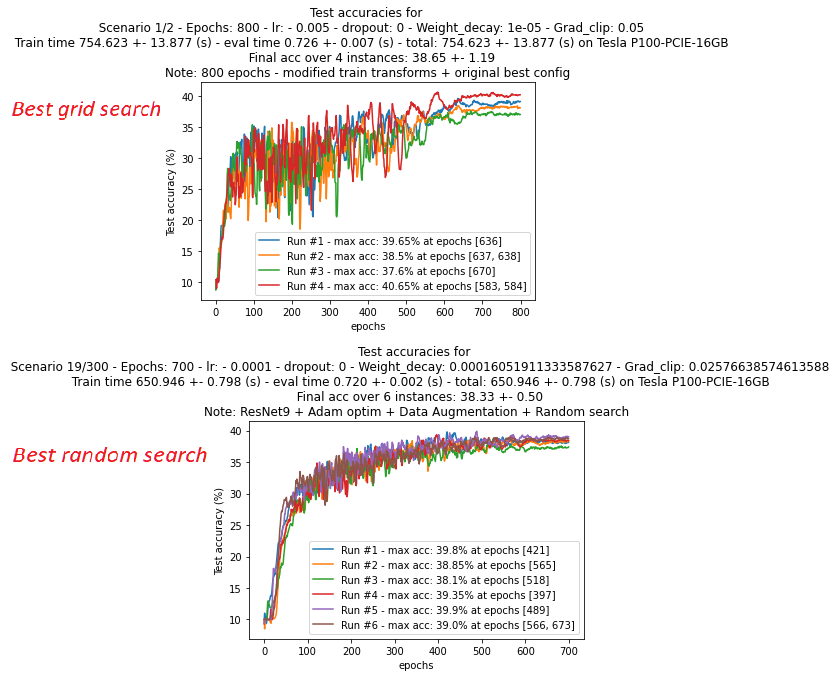
\includegraphics[width=1.1\linewidth]{img/REPORT_resnet9_Best_result_grid_vs_random_search.png}
   \caption{Improvement on ResNet-9 model performance from best grid search configuration (top) to best random search configuration (bottom). In the top image, despite reaching a similar final mean accuracy, the final accuracy standard deviation is higher than the bottom image, and more importantly, the high variation of the accuracy curves across 4 runs are much higher and hence gives hints of some uncertainty and less reliability in future runs on the test set in CodaLab.\label{figure:grid_vs_random}}
 \end{figure}

\subsubsection{Different approaches for challenge 1}

The team developed 3 different approaches, there results will be summarized in section \ref{subsubsection:challenge1_result}:
\paragraph{a) Traditional CNN models:} This has been the main approach mentioned from the beginning of this section  \ref{section:method-and-implementation}. We used the base ResNet-9 model with all of the techniques above and combined with the model performance evaluation method from the beginning. Moreover, we also tried different CNN models but could not reach the ResNet-9 performance as explained previously.
Thus, we submitted the ResNet-9 model as the final versions for both test bed and CodaLab.

\paragraph{b) Traditional linear models:} Despite the increasing deep learning field, traditional machine learning models are still proved to perform well enough in some situation so we would like to have a taste on how well they are in this limited data without pre-training challenge. 2 chosen models from the linear family are k-Nearest Neighbors (k-NN) and Support Vector Machine (SVM), because:

\begin{itemize}
    \item k-NN: k-NN has been known for a simple yet decent linear classifier which classification task can be performed directly without any training required. The only disadvantage of k-NN is scalability since it requires high computation resource to calculate pairwise distances of the predict point to the whole computation during predicting time. However, in such a limited data constraints like in this project's challenge, the computation resource is not matter, which made k-NN worth considering. In this project we implemented our own k-NN algorithm from PyTorch and Numpy libraries.
    \item SVM \cite{svm}: SVM is one of the best linear classifiers so far, with the powerful kernel functions that transform the data input space into non-linear space before the maximizing margin process. SVC classifier and RandomSearchCV from Skikit-Learn together form a great combination that can tackle basic image classification tasks on MNIST or CIFAR-10 datasets.
    
    For both algorithms, we used mini-batch multiplier and data augmentation to increase training sample sizes. Besides this, we could not use gradient descents related technique and just fine-tuning performance by grid search or auto random search. 
    The good thing is: both of them outperformed the given baseline CNN model. 
    
\end{itemize}

\paragraph{c) Hybrid approach - Deep metric learning using Triplet loss combined with a linear classifier (k-NN/SVM):}

The motivation for this approach come from the course's lab and assignment. One of the characteristic of deep metric learning is its suitability for learning few samples.  

Triplet loss is one of the more effective loss functions compared to pairwise (constrastive) loss.

From the idea that the distances of different class samples are pushed away from each other in embed space under the effect of the triplet loss, it will increase the chance for models like k-NN and SVM improve their prediction accuracy. Similar approaches are also seen from literature review \cite{AGARWAL2018_DAGSVM, tang13_dl_svm}, but in this method the author did make the SVM model differentiable why our team method is just utilize the SVM classifier from Skikit learn. 

Figure \ref{figure:challenge1_distances}

 \begin{figure*}[h!]
   \centering
       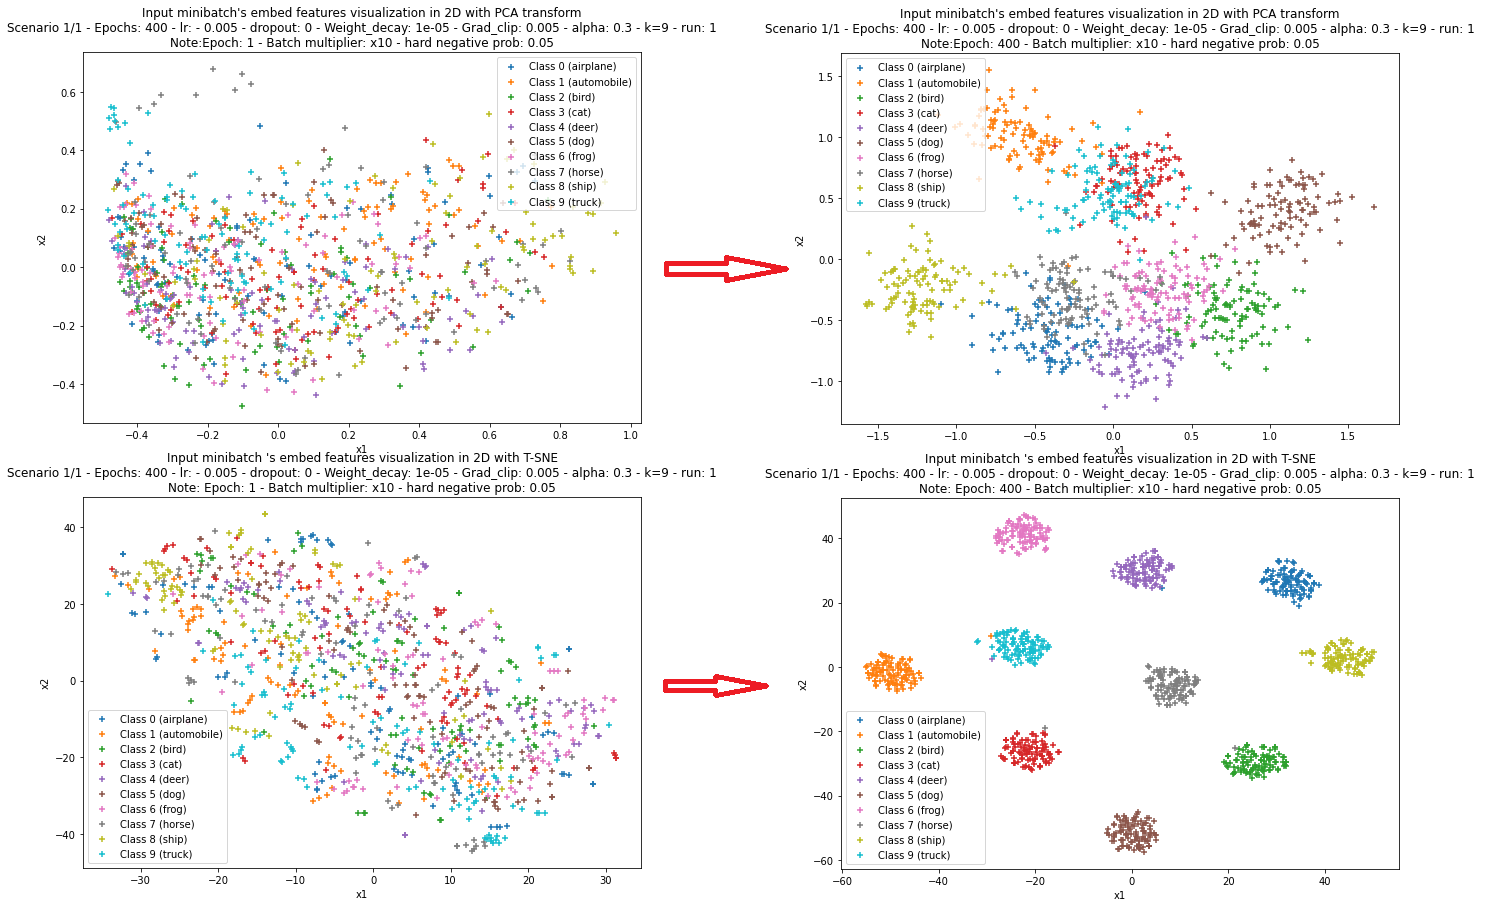
\includegraphics[width=0.9\linewidth]{img/REPORT_challenge1_triplet_distances.png}
   \caption{Visualization in 2D of input's embed space at the beging and after training completed for the hybrid approach in challenge 1. Left: distances at epoch 1 - Right: distances of after the final epoch - Top: PCA transformation - Bottom: T-SNE transformation. The triplet loss function helped push embeded points from different class away from each other, increased the classification chance for SVM, another margin-based optimization classifier.\label{figure:challenge1_distances}}
 \end{figure*}

Taking the good performance of the base model ResNet9, the final linear layer are removed to have the flatten layer (1028 features) to perform deep metric learning in embeded space during train time. When needed to perform training on the SVM or when need to make a prediction , the flatten layer will be connected with the SVM or k-NN classifier.

Here is a brief description of our implementation in this hybrid approach:

\hspace{0.2cm}- For each epoch, accumulate a few mini-batches of 100 samples (each already gone through random data argumentation), the number of batches are based on the pre-defined batch multiplier.

\hspace{0.2cm}- Generate triplets from the accumulated batch.

\hspace{0.2cm}- Split generated triplets into smaller batch again to train with the Triplet loss and Adam optimizer (applied all of the gradient related techniques in \ref{subsubsection:challenge1_techniques}).

\hspace{0.2cm}- During each epoch, can use k-NN (developed from Pytorch) to measure the validation accuracy.

\hspace{0.2cm}- At the final epoch, train the SVM classifier (from Scikit-learn) with the last accumulated batch using RandomSearchCV

\hspace{0.2cm}- After training complete, can either use the k-NN or the trained SVM to classify the validation set for final evaluation. (However, it could be observed during development phase that the SVM classifier most of the time performed better than the k-NN by 3-5\% when we tested the both prediction on the final epoch at the same time).

For triplet pairs generations, we follow the online mini-batch selection approach \cite{SchroffKP15_facenet}. In order to balance between execution time and performance, our team mixed between random triplet selection, hard and semi-hard negative mining in the following way:

\hspace{0.2cm}- When calling the triplet generation function for an accumulated batch input, the decision to whether perform random triplet selection or hard negative mining will be based on a random Bernoulli event (output 0 or 1) with an pre-defined probability \textit{p} (i.e. for p = 0.1, for each 400 running epochs will have approximately 40 epochs applied hard negative mining).

\hspace{0.2cm}- Due to the challenge of model collapse (loss function reach zero very early) \cite{kertesz20_metric_embedding}, for a given hard negative mining batch we mix randomly 40\% of semi-hard (i.e. for each 1000 samples in one accumulated batch, there would be around 400 samples selected with semi-hard negative criteria).

Our own hard-negative mining implementation is not optimal, which greatly impacted execution speed and could not have a good performance CodaLab submission. We also did not have enough time for fine-tuning the model, but it would be enough for the test bed version to achieve similar performance (a little bit lower) with the first approach (using purely ResNet-9 model) and still meet hard time constraints of 2 hours GPU run-time. 

Thus, we still submitted test bed code for this approach but not submitted in CodaLab.


\subsubsection{Result \& Discussion}
\label{subsubsection:challenge1_result}

Table \ref{table:result_challenge1} summarize our performance of different models and approaches.

The provided baseline CNN model in line 3 has the worst performance in term of test accuracy  mean and standard deviation. However, its execution times in Google Colab are the shortest due to the model's simplicity and no special technique applied. 

Due to the different test set in CodaLab and the evaluation on CodaLab sample size is larger (5000 samples versus 2000 samples in test bed), the variation (standard deviation) in the CodaLab runs is also expected to be higher than the test bed environment.

Surprisingly, linear models could perform better than the baseline CNN model. The k-NN model performed slightly better than the baseline CNN model with quite fast execution time, while the SVM classifier had a larger margin, in the expense of longer training time due to the implemented random search algorithm.

Our best performed model "\textbf{ResNet9 + Cosine Loss}" got the best accuracy in both Test bed and CodaLab environment. And with the accuracy curve met all of our defined criteria, it's reasonable why the variation across run in CodaLab was also very minimal. Execution time was also efficient enough with around 2.5 minutes (155 secs) although that is roughly 30x slower than the given baseline CNN model.

Other deeper models that we try with the same best config could not reach the performance from the ResNet9 model, even running with much longer time and more epochs, which could be explaned looking at their performance plots in the Appendix section.

Finally, our "thinking out of the box" hybrid approach and with the model "\textbf{ResNet9 + Triplet Loss + SVM}" could reach the same performance in both mean and std accuracy of the CNN ResNet9 model, but due to the limited time in optimizing code (especially in triplet hard negative selection phase) and limited fine-tuning time, it's current execution speed is much longer (20x slower) than the optimized ResNet9 CNN model, and the time variation is also big across runs due to unexpected behavior of current hard negative mining algorithm. Moreover, if we replace the SVM classifier by the k-NN one (just by simply change a parameter at the beginning of the Notebook), we can reduce training time by 5-6 minutes with the trade-offs of a few percents in accuracy decrease.     

\begin{table*}[h!]
    \caption{Performance summary of difference approaches and model in Challenge 1. Only models with high potential were tried submitting into CodaLab. At the end, 2 models "\textbf{ResNet9 + Cosine Loss}" and "\textbf{ResNet9 + Triplet Loss + SVM}" achieved the best performance and were selected to submit as final code (although only the CNN models approach was finally submitted for CodaLab evaluation).
    (*): numbers measured on running during developing phase on the train set similar to the initial test bed.
    (**): Estimated time calculated by subtracting average execution time of the last "\textbf{ResNet9 + Triplet Loss + SVM}" model by the average training time of the SVM classifier (since both classifiers are run at the same time with the same code during final evaluation test). 
    }
    \label{table:result_challenge1}
    \centering
    \begin{tabular}{|p{1.5cm}|p{3cm}|p{3cm}|p{3cm}|p{3cm}|p{1cm}|}
        \hline
        Approach & Model & Test Accuracy (Test Bed)  & Avg Run time (Testbed on Google Colab GPU) & Final Accuracy (CodaLab)  & Final submission\\

        \hline
       Linear models & k-NN (batch multiplier x10) & \(19.03 \pm 0.52\%\) (*) (over 3 instances) & \(\le20\) secs & N/A & No\\
       \hline
        Linear models & SVM (batch multiplier x10) & \(25.35 \pm 2.12\%\) (*) (over 3 instances) & \(1512 \pm 4.55\) secs  & N/A & No\\
        \hline
        CNN models & Baseline CNN (provided) & \(16.95 \pm 2.24\%\) (over 5 instances) & \(5.313 \pm 0.036\) secs & \(15.64 \pm 3.13\%\) (over 6 instances) & No \\
        
        \hline
        
        CNN models & \textbf{ResNet9 + Cosine Loss} & \textbf{38.88} \(\pm\) \textbf{2.86\%} & \(154.957 \pm 0.713\) secs & \textbf{37.95} \(\pm\) \textbf{0.35\%} (over 3 instances) & \textbf{Yes} (+ CodaLab)\\
 \hline
     CNN models & ResNet18 + Cosine Loss & 35.61 +- 1.02\% (*) (over 4 instances) & \(980.714 \pm 12.878\) secs & N/A  &    No\\
    \hline
    CNN models & ResNet50 + Cosine Loss & \(36.08 \pm 2.13\) (*) (over 4 instances) & \(2285.981 \pm 4.458\) secs  & \(0.2999 \pm 0.0149\%\) (over 2 instances)
 & No\\
    \hline
     CNN models& DenseNet + Cosine Loss & \(29.02 \pm 1.23\) & \(335.845 \pm 0.605\) secs  &  N/A & N/A \\
    \hline
    CNN models& ResNext14 & \(37.24 \pm 0.36\%\) (*) & \(927.815 \pm3.353\) secs & N/A & No\\
    \hline
    Hybrid models & ResNet9 + Triplet Loss + k-NN & \(36.5 \pm 3.05\%\)  (over 3 instances) & ~3252 secs (**)  & N/A & No\\
    \hline
    Hybrid models& \textbf{ResNet9 + Triplet Loss + SVM }& \(36.88 \pm 2.47\%\) (over 3 instances)& \(3652.571 \pm 620.558\) secs & N/A & \textbf{Yes} (No CodaLab) \\

    \hline
    \end{tabular}
\end{table*}


\subsection{Challenge 2}
\label{challenge2_subsection}
Transfer learning is a machine learning (ML) research problem that targets transfer knowledge gained  while solving one problem and applying it to a different but related problem. This knowledge transfer would improve the performance of learning and reduce 
the effort to recollect the data \cite{transfer-learning}. Different deep learning models that are composed of multiple layers to learn data such as Vgg16 from 
\cite{vgg16}, RestNet from \cite{Resnet50} , Alexnet from \cite{Alexnet} and EfficientNet from \cite{Efficientnet} can be used in advanced deep learning problems. In this challenge we are trying to use transfer learning to learn from limited data-set using different pre-trained models. we use a deep CNN with external data-set CINIC-10 \cite{cinic-10} for training our model to learn CIFAR-10 \cite{CIFAR-10} data-set classes. CINIC-10 dataset is constructed from two different sources: ImageNet and CIFAR-10. So, simply we removed all CIFAR samples from training and use only 1K samples per class for training purpose for the seek of limited the training time and resources. the best accuracy is around 86\%. 
\newline
The models we used are pre-trained on ImageNet dataset which contains large number of classes. the learned features from these deep models are very effective for small size datasets problems. AlexNet (Base Model), VGG16, RestNet-50 and EfficientNet-B0 are the models that we used for this challenge. For base-model, we just applied transfer of knowledge without being trained with external data. In the following sections we will discuss and analyze results.

\subsubsection{Reduce Over-fitting}
However, we apply feature extraction with each model and the performance is better than the baseline model (\~=50\%), there still exist hard overfitting due to lack of training samples. In order to reduce it, we used external dataset CINIC-10 with similar classes , implemented data augmentation and fine-tune with dropout.
\\\textbf{Data ugmentation sample for VGG16}\\
transforms.RandomResizedCrop(size=224,scale=(0.8,1.0)),\\
transforms.RandomRotation(degrees=15),\\
transforms.RandomHorizontalFlip(),\\
transforms.CenterCrop(size=224),\\
transforms.Normalize($[$0.485,0.456,0.406$]$,\newline$[$0.229,0.224,0.225$]$)
\\\\\textbf{Fine Tuning parameters for EfficientNet-B0:}
\begin{itemize}
\item DROPOUT\_RATE: 0.2
\item LR: 0.015
\item IMG\_SIZE: 224
\item RANDOMCROP: True
\item BATCHSIZE: 64
\item NUM\_EPOCHS : 30
\item WEIGHT\_DECAY: 0.0001
\end{itemize}

\subsubsection{Result & Discussion}
All experiments run on Google Colab Notebooks with virtual GPU. First, we download the CINIC-10 with only 1K sample/class from Github repository (link provided in notebook). Then we create training and validation directories to build the data loaders. We use accuracy and loss to decide the performance and over-fitting.

\\\textbf{Baseline Model:}
For the baseline, we directly run the provided pre-trained Alexnet model with 100 training sample and 2000 validation sample without any dropout or data augmentation to be compared with the following models as shallow model.
As can be seen from figure \ref{fig_base_model}, the baseline performs not well about 50\% validation accuracy and there exists strong over-fitting since training accuracy is much better than validation accuracy and validation loss value is greater than training loss value.
\begin{figure}[h]

\centering
\includegraphics[width=6 cm,height=5 cm]{img/image1.png}
\includegraphics[width=6 cm,height=5 cm]{img/image2.png}
\caption{ Baseline Model \label{fig_base_model}}
\end{figure}

\textbf{Feature extraction with models:}
Since we use pre-trained models, every downloaded model had modified to suites our dataset in terms of number of input channels and the output classifier number of classes. Because of limited resources, the number of training samples were bounded to CINIC-10 dataset (1K samples/class) + 10 samples /class from CIFAR10, the training time with GPU was under the bounded limit of 2 hours. The performance for each model is better than the baseline.

\textbf{Fine-tuning with models:}
In order to make better performance its recommended to fine-tune these models as well. For \textbf{VGG16} we unfreeze starting model layers by setting requires\_grad to False. For \textbf{EfficientNet-B0} we used pytorch implementation that 
cloned from github repo: 
\url{https://github.com/hirotomusiker/cifar10\_pytorch}. We applied some modification to make it suites our dataset also some hyper-parameters have changed by help of grid search to achieve higher accuracy i.e Learning rate changed from 0.01 to 0.015, batch size from 8 to 64, WEIGHT\_DECAY from 0.001 to 0.0001, IMAGE\_SIZE from 128 to 224 and finally drop out from 0.3 to 0.2.

\\\textbf{Trained Models Results:}
From \ref{fig_base_model}, it is too fast to get the result. it takes \~5 minutes per 30 epochs on CPU. However, the performance of this model is around 50\% for validation and 100\% for training. The training accuracy is much greater than validation accuracy and training loss value is much less than validation loss value. It is obvious that there exists strong overfitting since the training set size is very small (100 sample). 

\begin{figure}[h]

\centering
\includegraphics[width=6cm,height=5cm]{img/image3.png}
\includegraphics[width=6cm,height=5cm]{img/image4.png}
\caption{Vgg16 Model\label{fig_vgg16}}
\end{figure}

From \ref{fig_vgg16}, Vgg16 validation accuracy is greater than training accuracy, Also the training loss value is greater than validation value. Even though there is a little bit confusing but that means the model needs much training samples to generalize well which will violate the time limit allowed since VGG16 takes 65 minutes per 30 which will be doubled when increasing train data size. The validation accuracy also still near 72\%.

\begin{figure}[h]

\centering
\includegraphics[width=6cm,height=5cm]{img/image5.png}
\includegraphics[width=6cm,height=5cm]{img/image6.png}
\caption{ResNet 50 Model\label{fig_resnet50}}
\end{figure}

From \ref{fig_resnet50}, ResNet 50 training accuracy is less than validation accuracy and training loss value is much less than validation loss value that means there still exists overfitting in the model. the model needs much training samples to generalize well which will violate the time limit allowed. ResNet-50 takes 43 minutes per 30 epochs. The validation accuracy near also still near 71\%.

\begin{figure}[h]

\centering
\includegraphics[width=6cm,height=5cm]{img/image7.png}
\includegraphics[width=6cm,height=5cm]{img/image8.png}
\caption{Google EfficentNet-B0 Model\label{fig_efficientNetB0}}
\end{figure}

EfficientNets is a simple and highly effective compound scaling method, which enables us to easily scale up a baseline ConvNet to any target resource constraints in a more principled way, while maintaining model efficiency\cite{Efficientnet}.

From \ref{fig_efficientNetB0}, EfficientNet-B0 achieved the highest accuracy score for both training and validation in reasonable time. training accuracy is higher than validation accuracy. Also training loss value is higher than validation loss that means Model is learning well and able to generalize. the model may need much training samples and increasing number of epochs to achieve much higher accuracy. EfficientNet-B0 takes 40 minutes per 30 epochs to score validation accuracy near 86\% with less amount of resource in terms of GPU Memory. EfficientNet-B0 Model has run for 3 times for training and validation and achieve accuracy 83.77 -+ 2.30\% the following figure shows how accurate the model for inference.
\begin{figure}[h]

 \centering
 \includegraphics[width=6.30cm,height=6.19cm]{img/image9.png}
 \caption{Efficient Net Model Inference Output\label{fig_challange2_infer_results}}
\end{figure}

\textbf{Results Summary:} Table \ref{table:tbl_Transfer_learning_models_summary} summarizes the team's work on challenge 2. Our final submitted code is for model \textbf{EfficientNet B0} highlighted in \textbf{bold}


\begin{table*}[h!]
    \caption{Challenge 2 - Transfer learning models summary}
    \label{table:tbl_Transfer_learning_models_summary}
    \centering
    \begin{tabular}{|p{1.5cm}|p{2cm}|p{3cm}|p{1.5cm}|p{1cm}|p{1.5cm}|p{1cm}|p{1cm}|}
        \hline
        Approach & Model & Train Set & Test Set & Train Accuracy & Test Accuracy (TestBed) & Run time (Testbed /Google Colab) & Final submission \\
        \hline
        Transfer learning & Baseline (AlexNet) & 100 samples CIFAR-10 & 2K samples CIFAR-10 & ~99\% & 46.25 ± 6.72\% (1 CPU instance) & ~300 secs-Testbed & No \\
        \hline
        Transfer learning+ External Data & Vgg16 & 100 samples CIFAR-10 + 10K samples CINIC-10 & 2K samples CIFAR-10 & ~61\% & 70±1.25\% (1 GPU instance) & 3900 secs- Colab & No \\
        \hline
        Transfer learning+ External Data & ResNet50 & 100 samples CIFAR-10 + 10K samples CINIC-10 & 2K samples CIFAR-10 & ~70\% & 67±2.9\% (1 GPU instance) & 2580 secs- Colab & No \\
        \hline
        Transfer learning+ External Data & \textbf{EfficientNet B0} & 100 samples CIFAR-10 + 10K samples CINIC-10 & 2K samples CIFAR-10 & ~99\% & 83.77 ± 2.30\% (1 GPU instance) & 2400 secs- Colab & \textbf{Yes} \\
        \hline
    \end{tabular}
\end{table*}
%%%%%%%%%%%%%%%%%%%% Table No: 1 ends here %%%%%%%%%%%%%%%%%%%%


%------------------------------------------------------------------------
\section{Conclusions}

From this project, the team realized that learning from limited data is a very interesting but challenging experience.

In challenge 1, our team was able to perform well with the top result submission on CodaLab, as well as developed and implemented 2 models which give quite similar performance, although there are still things to be improve further if time allows (such as making the SVM classifier in  the third approach fully differentiable as in \cite{tang13_dl_svm}).

Learning with limited data without pre-trainning like in the challenge 1's context showed that regardless of the model and approach, the achieved performance is still below 50\% test accuracy, which proved than transfer learning approaches in challenge 2 are the proper way to conquer this kind of limited data challenge (excepted when the data in new domain has too much different characteristics compared to the source domain, where pre-trained approach would not help and the challenge 1's context is un-avoidable). 

For challenge 2, the objective is to show how deep models like VGG16, ResNet and EfficientNetB0 can be used on very small size data without large margin of overfitting and with great performance. All of the models are pre-trained on ImageNet. According to the experiments, most of the models had performed well, specially when apply data 
augmentation, dropout, and fine-tuning.

Overall, the experiments proved that deep models can be used to generalize well very small datasets with proper modifications and limited resources.
%In this work, we have successfully implemented Arithmetic coding and adapt some auto-regressive model to further improve the compression ratio. Comparing to popular data compression programs, our implementation achieve better result using dictionary (word level) but falls behind in term of real-world applications due to long running time. We also did not succeed in producing the fully working application (to output encoded bits to compressed file) but our codes only showed proof of concept of estimated compression time and ratio.  

%The compression ratio can be improved when we have enough resources to compress longer data sequences and pre-processing data more carefully. Meanwhile, run time performance can be improved using multi-thread implementation and using faster programming language such as C++. The size of vocabulary can also be improved by using \textit{subword units} \cite{sennrich-etal-2016-neural} without losing compression performance.


%Summarize what you could and could not conclude based on your experiments.

%The "References" section (bibliography) is optional. If you cite any books, websites, or academic papers, then you can add them to bibliography.bib and cite them in this report. Otherwise delete the references section.


{\small
\bibliographystyle{cvpr_bibstyle}
\bibliography{bibliography}
}


\newpage
\appendix


%-------------------------------------------------------------------------
\section*{Appendix}
\subsection{Member contributions}
\begin{itemize}
 \item Hussein: Initial ResNet9 model selection and first dev Notebook on Challenge 1; Developed and finished models in challenge 2; Meeting minutes taker. 
 \item Tuan: Implemented grid search and random search resuming mechanism and report features for challenge 1; Tried linear classifiers (2nd approach) in challenge 1; Implemented Triplet loss with k-NN/SVM classifier for approach 3; Roof reading on Challenge 2's submitted code; Meeting facilitators. 
 \item Dat: Fine-tuning ResNet9 models on challenge 1 using the provide grid and random search from Tuan; Explore deeper models' performance on challenge 1; Final code evaluation for challenge 2. 
\end{itemize}

\subsection{Additional images}
% \begin{figure}[h!]
%   \centering
%       \includegraphics[width=1.1\linewidth]{img/approach.png}
%   \caption{G17 project approach and framework\label{figure:approach}}
% \end{figure}

\begin{figure}[h!]
   \centering
       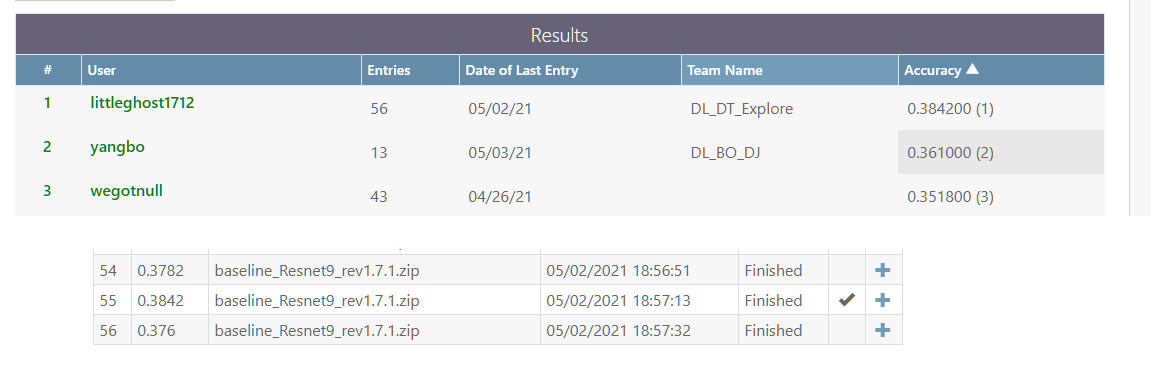
\includegraphics[width=1.2\linewidth]{img/APPENDIX_CodaLab_dashboard.png}
   \caption{CodaLab competition dashboard for challenge 1. Our team is \textbf{DL\_DT\_Explore} and below table are the results of 3 run for our final submission\label{figure:CodaLab}}
 \end{figure}
 
 \begin{figure}[h!]
   \centering
       \includegraphics[width=1.1\linewidth]{img/APPENDIX_challenge1_data_aug_settings.png}
   \caption{Best data augmentation settings for challenge 1\label{figure:data_aug_setting_challenge1}}
 \end{figure}
 
 \begin{figure}[h!]
   \centering
       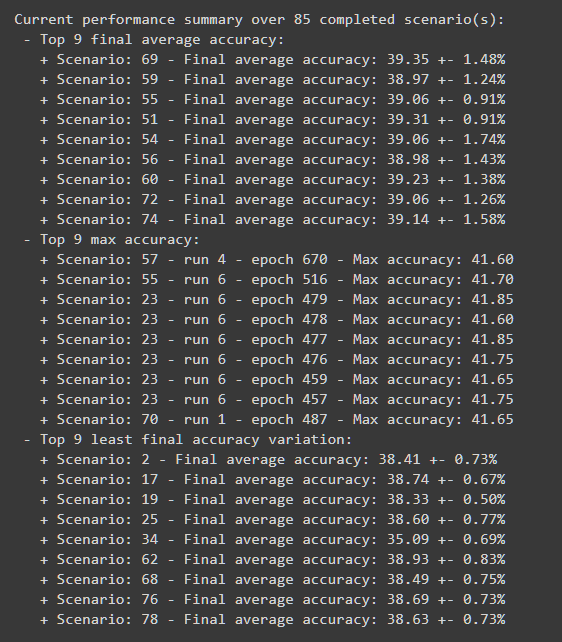
\includegraphics[width=1.1\linewidth]{img/APPENDIX_performance_summary_sample.png}
   \caption{Performance tracking and summary result output (used for grid search or random search). Our best performance settings was from scenario 9 from the summary\label{figure:summary_track}}
 \end{figure}

 \begin{figure}[h!]
   \centering
       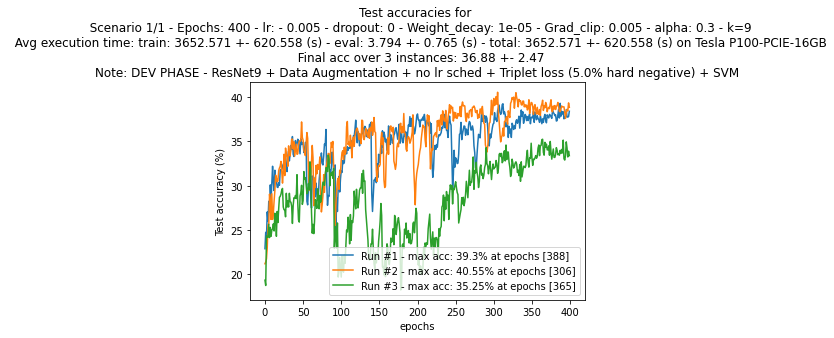
\includegraphics[width=1.1\linewidth]{img/APENDIX_Triplet_SVM_result.png}
   \caption{Performance of the hybrid approach: \textbf{ResNet9 + Triplet Loss + SVM }. We did not have enough time for fine-tuning this model\label{figure:triplet_svm_curves}}
 \end{figure}

 \begin{figure}[h!]

       \includegraphics[width=1.1\linewidth]{img/APPENDIX_DenseNet_results.png}
   \caption{Best performance of DenseNet model\label{figure:densenet}}
 \end{figure} 

 \begin{figure}[h!]

       \includegraphics[width=1.1\linewidth]{img/APPENDIX_resnet18_best_result.png}
   \caption{Best performance of ResNet-18 model\label{figure:resnet18}}
 \end{figure}
 
 \begin{figure}[h!]

       \includegraphics[width=1.1\linewidth]{img/APPENDIX_resnet50_best_result.png}
   \caption{Best performance of ResNet-50 model\label{figure:resnet50}}
 \end{figure}

 \begin{figure}[h!]

       \includegraphics[width=1.1\linewidth]{img/APPENDIX_resnext14_best_performance.png}
   \caption{Best performance of ResNext-14 model\label{figure:resnext14}}
 \end{figure} 

% DELETE THIS TEXT
%If you want to include extra more detailed results that did not fit within the main report, include them here. Or, you can just delete this example section.

%-------------------------------------------------------------------------
%\section*{Appendix: Examples of \LaTeX}

% % The 'dilde' in Table~\ref{} puts a no-break space prevents "Table" and "1" so that
% % the table number does not get split onto a separate line.
% % and it is good LaTeX practice to put tildes between 

% % DELETE THIS TEXT
% This section contains some examples of \LaTeX~to help you get started.
% (You should delete this section in the final report.)
% This is a reference to Table~\ref{first_table} and Table~\ref{second_table}.
% This is a reference to Figure~\ref{first_figure} and Figure~\ref{second_figure}.
% This is a citation \cite{breiman2001statistical} and this is
% multiple citations \cite{breiman2001statistical,bishop2006pattern}.
% This is \textit{italics} and \textbf{bold} text.
% This is a formula $\sum_{i=1}^N (y_i - \hat{y}_i(\mathbf{x}))^2$
% that is inline with the text (`text style') and this is a
% formula that is displayed separately (`display style'):
% $$
% \sum_{i=1}^N (y_i - \hat{y}_i(\mathbf{x}))^2
% $$
% These are formulas with an associated equation number
% \begin{align}
%   \mathbf{x} = \begin{bmatrix}
%       x_1, x_2, \ldots, x_N
%   \end{bmatrix}^T    \label{xvec}\\
%   \boldsymbol{\phi} = \begin{bmatrix}
%       \phi_1, \phi_2, \ldots, \phi_M
%   \end{bmatrix}^T    \label{phivec}
% \end{align}
% and we can now refer back to~\eqref{xvec} or to ~\eqref{phivec} like so.



% % DELETE THIS TABLE
% \begin{table}
%   \begin{center}
%   \begin{tabular}{|l|c|c|}
%   \hline
%   Method & Ultra-Clustering & Random Jungles \\
%   \hline\hline
%   Theirs & Works OK & All your base\\
%   Yours & Works better & are belong to us!\\
%   Ours & Works best! & I can haz publication?\\
%   \hline
%   \end{tabular}
%   \end{center}
%   \caption{This is the caption of a column-width table.\label{first_table}}
% \end{table}

% % DELETE THIS TABLE
% \begin{table*}
%   \begin{center}
%   \begin{tabular}{|l|c|c|c|}
%   \hline
%   Method & Good? & Bad? & So-so? \\
%   \hline\hline
%   Your method & Terrible & Yes, I made sure of it & Star Wars movies \\
%   My supervisor's old method (sigh) & I want Tim Horton's & People in hallway... & ...are talking too loudly \\
%   My proposed method  & Yes, good! & No, I said good! & What? \\
%   \hline
%   \end{tabular}
%   \end{center}
%   \caption{This is the caption of a page-width table.\label{second_table}}
% \end{table*}


% % DELETE THIS FIGURE
% \begin{figure}
%   \begin{center}
%   \includegraphics[width=\linewidth]{sample_image.png}
%   \end{center}
%       \caption{This is the caption of a column-width figure.\label{first_figure}}
% \end{figure}
   

% % DELETE THIS FIGURE
% \begin{figure*}
%   \begin{center}
%       \includegraphics[width=0.4\linewidth]{sample_image.pdf}
%       \includegraphics[width=0.4\linewidth]{sample_image.pdf}
%   \end{center}
%       \caption{This is the caption of a page-width figure.\label{second_figure}}
% \end{figure*}




\end{document}
